\documentclass[10pt,ignorenonframetext,compress, aspectratio=169]{beamer}
\usetheme{m}
\usefonttheme[onlymath]{serif}
\setbeamertemplate{caption}[numbered]
\setbeamertemplate{caption label separator}{:}
\setbeamercolor{caption name}{fg=normal text.fg}
\usepackage{amssymb,amsmath}
% mathtools for underbracket
\usepackage{mathtools}
% \usepackage{ifxetex,ifluatex} % m theme needs xelatex
\usepackage{fixltx2e} % provides \textsubscript
% \usepackage{lmodern} kills bullets m theme
% \ifxetex
  \usepackage{fontspec,xltxtra,xunicode}
  \defaultfontfeatures{Mapping=tex-text,Scale=MatchLowercase}
  \newcommand{\euro}{€}
% \else
%   \ifluatex
%     \usepackage{fontspec}
%     \defaultfontfeatures{Mapping=tex-text,Scale=MatchLowercase}
%     \newcommand{\euro}{€}
%   \else
%     \usepackage[T1]{fontenc}
%     \usepackage[utf8]{inputenc}
%     %   \fi
% \fi
% use upquote if available, for straight quotes in verbatim environments
\IfFileExists{upquote.sty}{\usepackage{upquote}}{}
% use microtype if available
\IfFileExists{microtype.sty}{\usepackage{microtype}}{}
\usepackage{color}
\usepackage{fancyvrb}
\newcommand{\VerbBar}{|}
\newcommand{\VERB}{\Verb[commandchars=\\\{\}]}
\DefineVerbatimEnvironment{Highlighting}{Verbatim}{commandchars=\\\{\}}
% Add ',fontsize=\small' for more characters per line
\usepackage{framed}
\definecolor{shadecolor}{RGB}{248,248,248}
\newenvironment{Shaded}{\begin{snugshade}}{\end{snugshade}}
\newcommand{\KeywordTok}[1]{\textcolor[rgb]{0.13,0.29,0.53}{\textbf{{#1}}}}
\newcommand{\DataTypeTok}[1]{\textcolor[rgb]{0.13,0.29,0.53}{{#1}}}
\newcommand{\DecValTok}[1]{\textcolor[rgb]{0.00,0.00,0.81}{{#1}}}
\newcommand{\BaseNTok}[1]{\textcolor[rgb]{0.00,0.00,0.81}{{#1}}}
\newcommand{\FloatTok}[1]{\textcolor[rgb]{0.00,0.00,0.81}{{#1}}}
\newcommand{\CharTok}[1]{\textcolor[rgb]{0.31,0.60,0.02}{{#1}}}
\newcommand{\StringTok}[1]{\textcolor[rgb]{0.31,0.60,0.02}{{#1}}}
\newcommand{\CommentTok}[1]{\textcolor[rgb]{0.56,0.35,0.01}{\textit{{#1}}}}
\newcommand{\OtherTok}[1]{\textcolor[rgb]{0.56,0.35,0.01}{{#1}}}
\newcommand{\AlertTok}[1]{\textcolor[rgb]{0.94,0.16,0.16}{{#1}}}
\newcommand{\FunctionTok}[1]{\textcolor[rgb]{0.00,0.00,0.00}{{#1}}}
\newcommand{\RegionMarkerTok}[1]{{#1}}
\newcommand{\ErrorTok}[1]{\textbf{{#1}}}
\newcommand{\NormalTok}[1]{{#1}}

% Comment these out if you don't want a slide with just the
% part/section/subsection/subsubsection title:
% \AtBeginPart{
%   \let\insertpartnumber\relax
%   \let\partname\relax
%   \frame{\partpage}
% }
% \AtBeginSection{
%   \let\insertsectionnumber\relax
%   \let\sectionname\relax
%   \frame{\sectionpage}
% }
% \AtBeginSubsection{
%   \let\insertsubsectionnumber\relax
%   \let\subsectionname\relax
%   \frame{\subsectionpage}
% }

\setlength{\parindent}{0pt}
\setlength{\parskip}{6pt plus 2pt minus 1pt}
\setlength{\emergencystretch}{3em}  % prevent overfull lines
\setcounter{secnumdepth}{0}

% Textcomp for various common symbols
\usepackage{textcomp}

\usepackage{booktabs}

% Creative Commons Icons
\usepackage[scale=2]{ccicons}

\newenvironment{centrefig}{\begin{figure}\centering}{\end{figure}}
\newcommand{\columnsbegin}{\begin{columns}}
\newcommand{\columnsend}{\end{columns}}
\newcommand{\centreFigBegin}{\begin{columns}\centering}
\newcommand{\centreFigEnd}{\end{figure}}


\title{A Brief Introduction to R}
\author{Gavin L. Simpson}
\date{CSEE 2015 • May 20th 2015}

\begin{document}
\frame{\titlepage}

\begin{frame}[fragile]

\begin{verbatim}
Loading required package: methods
Loading required package: grid
\end{verbatim}

\end{frame}

\begin{frame}{Why R?}

Why use a complicated, command-line driven stats package like R?

\begin{itemize}
\itemsep1pt\parskip0pt\parsep0pt
\item
  It's free!
\item
  Widley used by statisticians for new statistical methods
\item
  If something doesn't work the way you like, you can change it
\item
  R is a programming language --- you can write your own functions
\item
  R scripts, \alert{Sweave}, \& \alert{knitr} for reproducible research
\item
  Works everywhere (Windows, OS X, Linux, \ldots{})
\item
  R was designed for expressive data analysis
\end{itemize}

\end{frame}

\section{R Basics}\label{r-basics}

\begin{frame}{R Basics}

Start \alert{RStudio} --- take a look around

R will be running in either your home directory or where is was
installed

Set the working directory to folder containing your analysis

\end{frame}

\begin{frame}{Getting Help}

R comes with a lot of documentation

To get help on functions or concepts within R, use the \texttt{"?"}
operator

For help on the \texttt{getwd()} function use: \texttt{?getwd}

Function \texttt{help.search("foo")} will search through all packages
installed for help pages with \texttt{foo} in them

R-Help mailing list: \url{http://www.r-project.org/mail.html}

\end{frame}

\begin{frame}{Getting Help: Task Views}

\url{cran.r-project.org/web/views/}

\begin{figure}
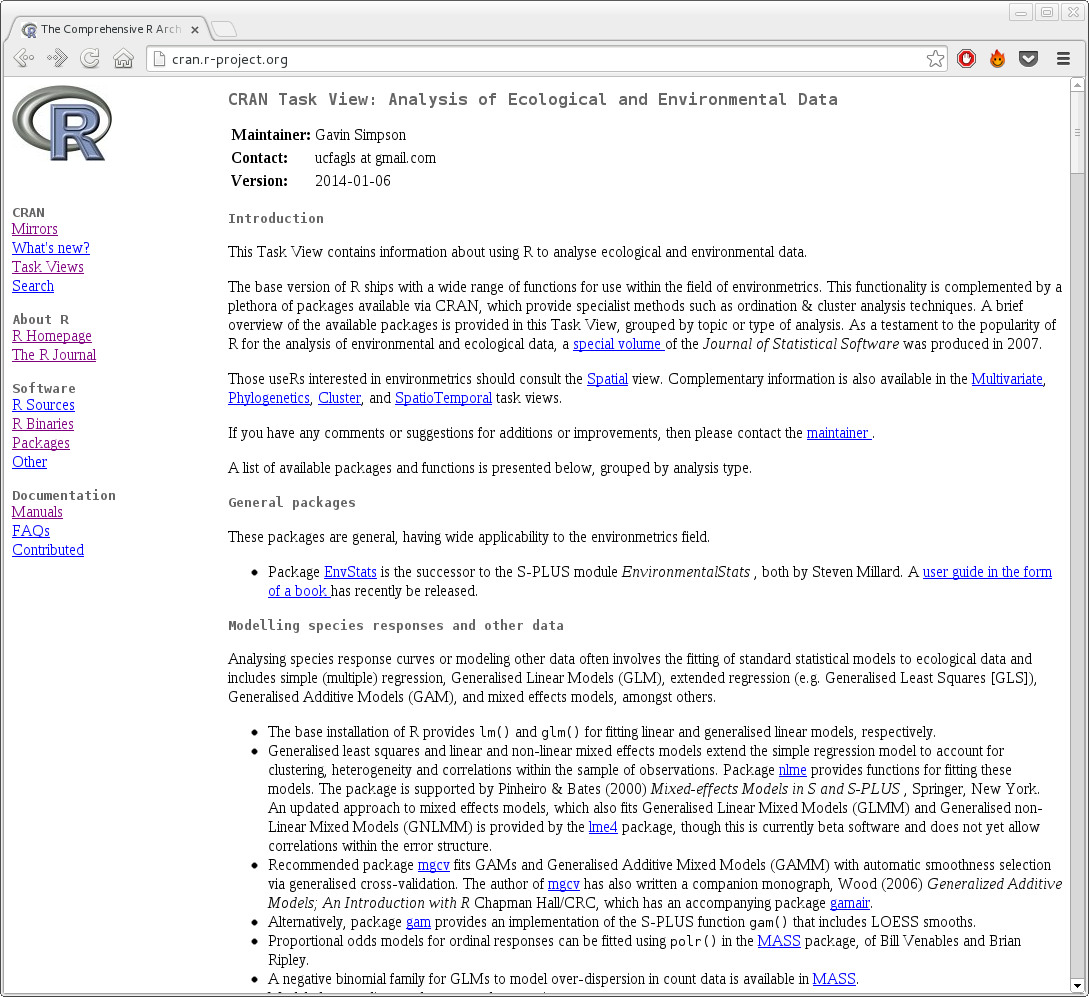
\includegraphics[height=6cm,keepaspectratio=true]{figs/cran-task-views}
\end{figure}

\end{frame}

\begin{frame}{Getting Help: Stack Overflow}

\url{stackoverflow.com/questions/tagged/r}

\begin{figure}

\includegraphics[height=6cm,keepaspectratio=true]{figs/stackoverflow-screen-grab}
\end{figure}

\end{frame}

\begin{frame}[fragile]{Working with R}

Type commands at the prompt \texttt{\textgreater{}} --- R evaluates them
when you hit \texttt{Return}

If a line is \emph{not} syntactically complete, the prompt changes to
\texttt{+}

Create an object by assigning something to it

\scriptsize

\begin{Shaded}
\begin{Highlighting}[]
\NormalTok{radius <-}\StringTok{ }\DecValTok{5}
\NormalTok{pi *}\StringTok{ }\NormalTok{radius^}\DecValTok{2}
\end{Highlighting}
\end{Shaded}

\begin{verbatim}
[1] 78.53982
\end{verbatim}

\normalsize

If we don't assign, R prints a \emph{representation} of the object

\end{frame}

\begin{frame}[fragile]{Packages}

R comes with a basic set of functionality plus some \alert{reccomended}
packages

Additional functionality added via \alert{packages} from \textbf{CRAN},
\textbf{github}, \textbf{Bioconductor}, \textbf{drat} repos

\scriptsize

\begin{Shaded}
\begin{Highlighting}[]
\KeywordTok{install.packages}\NormalTok{(}\KeywordTok{c}\NormalTok{(}\StringTok{"gapminder"}\NormalTok{, }\StringTok{"ggplot2"}\NormalTok{))}
\KeywordTok{library}\NormalTok{(}\StringTok{"gapminder"}\NormalTok{)}
\KeywordTok{library}\NormalTok{(}\StringTok{"ggplot2"}\NormalTok{)}
\end{Highlighting}
\end{Shaded}

\normalsize

\end{frame}

\begin{frame}[fragile]{Reading data into R}

\scriptsize

\begin{Shaded}
\begin{Highlighting}[]
\NormalTok{gap <-}\StringTok{ }\KeywordTok{system.file}\NormalTok{(}\StringTok{"gapminder.tsv"}\NormalTok{, }\DataTypeTok{package =} \StringTok{"gapminder"}\NormalTok{)}
\NormalTok{gapminder <-}\StringTok{ }\KeywordTok{read.delim}\NormalTok{(gap)}
\KeywordTok{head}\NormalTok{(gapminder)}
\end{Highlighting}
\end{Shaded}

\begin{verbatim}
      country continent year lifeExp      pop gdpPercap
1 Afghanistan      Asia 1952  28.801  8425333  779.4453
2 Afghanistan      Asia 1957  30.332  9240934  820.8530
3 Afghanistan      Asia 1962  31.997 10267083  853.1007
4 Afghanistan      Asia 1967  34.020 11537966  836.1971
5 Afghanistan      Asia 1972  36.088 13079460  739.9811
6 Afghanistan      Asia 1977  38.438 14880372  786.1134
\end{verbatim}

\normalsize

\end{frame}

\begin{frame}[fragile]{This is where we are heading}

\scriptsize

\begin{Shaded}
\begin{Highlighting}[]
\KeywordTok{ggplot}\NormalTok{(}\KeywordTok{subset}\NormalTok{(gapminder, continent !=}\StringTok{ "Oceania"}\NormalTok{),}
       \KeywordTok{aes}\NormalTok{(}\DataTypeTok{x =} \NormalTok{year, }\DataTypeTok{y =} \NormalTok{lifeExp, }\DataTypeTok{group =} \NormalTok{country, }\DataTypeTok{color =} \NormalTok{country)) +}
\StringTok{  }\KeywordTok{geom_line}\NormalTok{(}\DataTypeTok{show_guide =} \OtherTok{FALSE}\NormalTok{) +}\StringTok{ }\KeywordTok{facet_wrap}\NormalTok{(~}\StringTok{ }\NormalTok{continent) +}
\StringTok{  }\KeywordTok{scale_color_manual}\NormalTok{(}\DataTypeTok{values =} \NormalTok{country_colors) +}
\StringTok{  }\KeywordTok{theme_bw}\NormalTok{()}
\end{Highlighting}
\end{Shaded}

\begin{center}\includegraphics[width=0.6\linewidth]{intro-r-slides_files/figure-beamer/gapminder-example-1} \end{center}

\normalsize

\end{frame}

\begin{frame}[fragile]{R Objects}

What kind of object is \texttt{gapminder}?

\scriptsize

\begin{Shaded}
\begin{Highlighting}[]
\KeywordTok{str}\NormalTok{(gapminder)}
\end{Highlighting}
\end{Shaded}

\begin{verbatim}
'data.frame':   1704 obs. of  6 variables:
 $ country  : Factor w/ 142 levels "Afghanistan",..: 1 1 1 1 1 1 1 1 1 1 ...
 $ continent: Factor w/ 5 levels "Africa","Americas",..: 3 3 3 3 3 3 3 3 3 3 ...
 $ year     : int  1952 1957 1962 1967 1972 1977 1982 1987 1992 1997 ...
 $ lifeExp  : num  28.8 30.3 32 34 36.1 ...
 $ pop      : num  8425333 9240934 10267083 11537966 13079460 ...
 $ gdpPercap: num  779 821 853 836 740 ...
\end{verbatim}

\begin{Shaded}
\begin{Highlighting}[]
\KeywordTok{class}\NormalTok{(gapminder)}
\end{Highlighting}
\end{Shaded}

\begin{verbatim}
[1] "data.frame"
\end{verbatim}

\normalsize

\end{frame}

\begin{frame}{Data frames}

A \alert{data frame} is R's version of an Excel spreadsheet

Columns are variables

Rows are observations

Different \textbf{types} of data in columns

Each column (\alert{component}) is of the same length

Is a special case of a list

\end{frame}

\begin{frame}[fragile]{Subsetting}

Access the columns of a data frame using \texttt{{[}}, \texttt{{[}{[}}
or \texttt{\$}

\texttt{\$} is simple:

Access just a single variable

\scriptsize

\begin{Shaded}
\begin{Highlighting}[]
\KeywordTok{head}\NormalTok{(gapminder$country)}
\end{Highlighting}
\end{Shaded}

\begin{verbatim}
[1] Afghanistan Afghanistan Afghanistan Afghanistan Afghanistan Afghanistan
142 Levels: Afghanistan Albania Algeria Angola Argentina ... Zimbabwe
\end{verbatim}

\normalsize

Uses the name of required variable

Partial matching

\scriptsize

\begin{Shaded}
\begin{Highlighting}[]
\KeywordTok{head}\NormalTok{(gapminder$cou)}
\end{Highlighting}
\end{Shaded}

\begin{verbatim}
[1] Afghanistan Afghanistan Afghanistan Afghanistan Afghanistan Afghanistan
142 Levels: Afghanistan Albania Algeria Angola Argentina ... Zimbabwe
\end{verbatim}

\normalsize

\end{frame}

\begin{frame}[fragile]{Subsetting}

\texttt{{[}{[}} is a little more flexible:

Access just a single variable

Use the name of required variable

\scriptsize

\begin{Shaded}
\begin{Highlighting}[]
\KeywordTok{head}\NormalTok{(gapminder[[}\StringTok{"continent"}\NormalTok{]])}
\end{Highlighting}
\end{Shaded}

\begin{verbatim}
[1] Asia Asia Asia Asia Asia Asia
Levels: Africa Americas Asia Europe Oceania
\end{verbatim}

\normalsize

Or select the \emph{n}th component

\scriptsize

\begin{Shaded}
\begin{Highlighting}[]
\KeywordTok{head}\NormalTok{(gapminder[[}\DecValTok{2}\NormalTok{]])}
\end{Highlighting}
\end{Shaded}

\begin{verbatim}
[1] Asia Asia Asia Asia Asia Asia
Levels: Africa Americas Asia Europe Oceania
\end{verbatim}

\normalsize

Partial matching optional ---
\texttt{gapminder{[}{[}"cont", exact = FALSE{]}{]}}

\end{frame}

\begin{frame}[fragile]{Subsetting}

\texttt{{[}} is a even more flexible:

Access one or more variables

Use the name(s) of required variable

\scriptsize

\begin{Shaded}
\begin{Highlighting}[]
\KeywordTok{head}\NormalTok{(gapminder[}\KeywordTok{c}\NormalTok{(}\StringTok{"country"}\NormalTok{, }\StringTok{"continent"}\NormalTok{)])}
\end{Highlighting}
\end{Shaded}

\begin{verbatim}
      country continent
1 Afghanistan      Asia
2 Afghanistan      Asia
3 Afghanistan      Asia
4 Afghanistan      Asia
5 Afghanistan      Asia
6 Afghanistan      Asia
\end{verbatim}

\normalsize

\end{frame}

\begin{frame}[fragile]{subsetting}

Or select the \emph{n}th component(s)

\scriptsize

\begin{Shaded}
\begin{Highlighting}[]
\KeywordTok{head}\NormalTok{(gapminder[}\DecValTok{1}\NormalTok{:}\DecValTok{2}\NormalTok{])}
\end{Highlighting}
\end{Shaded}

\begin{verbatim}
      country continent
1 Afghanistan      Asia
2 Afghanistan      Asia
3 Afghanistan      Asia
4 Afghanistan      Asia
5 Afghanistan      Asia
6 Afghanistan      Asia
\end{verbatim}

\normalsize

\end{frame}

\begin{frame}[fragile]{subsetting}

Or we can index by rows and columns:
\texttt{{[}rows, cols, other\_args{]}}

\scriptsize

\begin{Shaded}
\begin{Highlighting}[]
\KeywordTok{head}\NormalTok{(gapminder[}\DecValTok{1}\NormalTok{:}\DecValTok{4}\NormalTok{, }\KeywordTok{c}\NormalTok{(}\DecValTok{1}\NormalTok{,}\DecValTok{3}\NormalTok{)])}
\end{Highlighting}
\end{Shaded}

\begin{verbatim}
      country year
1 Afghanistan 1952
2 Afghanistan 1957
3 Afghanistan 1962
4 Afghanistan 1967
\end{verbatim}

\normalsize

\end{frame}

\begin{frame}[fragile]{subsetting}

Leaving the row or column identifier \emph{blank} means \textbf{``give
me all of the rows (columns)''}

\scriptsize

\begin{Shaded}
\begin{Highlighting}[]
\KeywordTok{head}\NormalTok{(gapminder[}\DecValTok{1}\NormalTok{:}\DecValTok{4}\NormalTok{, ])                  }\CommentTok{# all columns, rows 1--4}
\end{Highlighting}
\end{Shaded}

\begin{verbatim}
      country continent year lifeExp      pop gdpPercap
1 Afghanistan      Asia 1952  28.801  8425333  779.4453
2 Afghanistan      Asia 1957  30.332  9240934  820.8530
3 Afghanistan      Asia 1962  31.997 10267083  853.1007
4 Afghanistan      Asia 1967  34.020 11537966  836.1971
\end{verbatim}

\normalsize

\scriptsize

\begin{Shaded}
\begin{Highlighting}[]
\KeywordTok{head}\NormalTok{(gapminder[, }\DecValTok{1}\NormalTok{:}\DecValTok{3}\NormalTok{], }\DecValTok{3}\NormalTok{)               }\CommentTok{# all rows, columns 1--3}
\end{Highlighting}
\end{Shaded}

\begin{verbatim}
      country continent year
1 Afghanistan      Asia 1952
2 Afghanistan      Asia 1957
3 Afghanistan      Asia 1962
\end{verbatim}

\normalsize

\end{frame}

\begin{frame}[fragile]{subsetting}

Empty dimensions get \textbf{dropped} if you select a single column

\scriptsize

\begin{Shaded}
\begin{Highlighting}[]
\KeywordTok{head}\NormalTok{(gapminder[, }\DecValTok{2}\NormalTok{], }\DecValTok{3}\NormalTok{)                 }\CommentTok{# just column 2}
\end{Highlighting}
\end{Shaded}

\begin{verbatim}
[1] Asia Asia Asia
Levels: Africa Americas Asia Europe Oceania
\end{verbatim}

\normalsize

Preserve dimensions using \texttt{drop = FALSE}

\scriptsize

\begin{Shaded}
\begin{Highlighting}[]
\KeywordTok{head}\NormalTok{(gapminder[, }\DecValTok{2}\NormalTok{, }\DataTypeTok{drop =} \OtherTok{FALSE}\NormalTok{], }\DecValTok{3}\NormalTok{)   }\CommentTok{# all rows, columns 1--3}
\end{Highlighting}
\end{Shaded}

\begin{verbatim}
  continent
1      Asia
2      Asia
3      Asia
\end{verbatim}

\normalsize

\end{frame}

\begin{frame}[fragile]{Subsetting}

Can use a range of \alert{index} types

\begin{itemize}
\itemsep1pt\parskip0pt\parsep0pt
\item
  Numeric values select the \texttt{n}th elements
\item
  Negative numeric values select all but those elements
\item
  Character values select elements by name (possibly with partial
  matching)
\item
  Logical values select (\texttt{TRUE}) \& deselect (\texttt{FALSE})
  elements
\item
  Logical indices are \alert{recycled} to the correct length
\end{itemize}

\scriptsize

\begin{Shaded}
\begin{Highlighting}[]
\NormalTok{(}\DecValTok{1}\NormalTok{:}\DecValTok{10}\NormalTok{)[}\KeywordTok{c}\NormalTok{(}\OtherTok{FALSE}\NormalTok{, }\OtherTok{TRUE}\NormalTok{)]}
\end{Highlighting}
\end{Shaded}

\begin{verbatim}
[1]  2  4  6  8 10
\end{verbatim}

\begin{Shaded}
\begin{Highlighting}[]
\NormalTok{(}\DecValTok{1}\NormalTok{:}\DecValTok{9}\NormalTok{)[}\KeywordTok{c}\NormalTok{(}\OtherTok{FALSE}\NormalTok{, }\OtherTok{TRUE}\NormalTok{)]                   }\CommentTok{# no warning}
\end{Highlighting}
\end{Shaded}

\begin{verbatim}
[1] 2 4 6 8
\end{verbatim}

\normalsize

\end{frame}

\begin{frame}[fragile]{Vectors}

What are the columns of \texttt{gapminder}?

\scriptsize

\begin{Shaded}
\begin{Highlighting}[]
\KeywordTok{str}\NormalTok{(gapminder)}
\end{Highlighting}
\end{Shaded}

\begin{verbatim}
'data.frame':   1704 obs. of  6 variables:
 $ country  : Factor w/ 142 levels "Afghanistan",..: 1 1 1 1 1 1 1 1 1 1 ...
 $ continent: Factor w/ 5 levels "Africa","Americas",..: 3 3 3 3 3 3 3 3 3 3 ...
 $ year     : int  1952 1957 1962 1967 1972 1977 1982 1987 1992 1997 ...
 $ lifeExp  : num  28.8 30.3 32 34 36.1 ...
 $ pop      : num  8425333 9240934 10267083 11537966 13079460 ...
 $ gdpPercap: num  779 821 853 836 740 ...
\end{verbatim}

\normalsize

Each component is a vector, of which there are several types:
\texttt{numeric}, \texttt{character}, \texttt{logical}, \texttt{factor},
\texttt{integer}

\end{frame}

\begin{frame}[fragile]{Vectors --- numeric \& integer}

R normally stores numeric data as \emph{doubles} (decimal values)

There is an \emph{integer} type too

\scriptsize

\begin{Shaded}
\begin{Highlighting}[]
\KeywordTok{class}\NormalTok{(gapminder$lifeExp)}
\end{Highlighting}
\end{Shaded}

\begin{verbatim}
[1] "numeric"
\end{verbatim}

\begin{Shaded}
\begin{Highlighting}[]
\KeywordTok{class}\NormalTok{(gapminder$year)}
\end{Highlighting}
\end{Shaded}

\begin{verbatim}
[1] "integer"
\end{verbatim}

\normalsize

\end{frame}

\begin{frame}[fragile]{Vectors --- numeric \& integer}

Create numeric vectors using \texttt{c()} or \texttt{:}

\scriptsize

\begin{Shaded}
\begin{Highlighting}[]
\KeywordTok{c}\NormalTok{(}\DecValTok{1}\NormalTok{,}\DecValTok{3}\NormalTok{,}\DecValTok{5}\NormalTok{,}\DecValTok{7}\NormalTok{,}\DecValTok{9}\NormalTok{)}
\end{Highlighting}
\end{Shaded}

\begin{verbatim}
[1] 1 3 5 7 9
\end{verbatim}

\begin{Shaded}
\begin{Highlighting}[]
\DecValTok{1}\NormalTok{:}\DecValTok{10}
\end{Highlighting}
\end{Shaded}

\begin{verbatim}
 [1]  1  2  3  4  5  6  7  8  9 10
\end{verbatim}

\normalsize

\texttt{x:y} is shorthand for \texttt{seq(from = x, to = y, by = 1)}

\end{frame}

\begin{frame}[fragile]{Vectors --- character}

Character vectors contain text (strings)

\scriptsize

\begin{Shaded}
\begin{Highlighting}[]
\KeywordTok{c}\NormalTok{(}\StringTok{"foo"}\NormalTok{,}\StringTok{"bar"}\NormalTok{)}
\end{Highlighting}
\end{Shaded}

\begin{verbatim}
[1] "foo" "bar"
\end{verbatim}

\normalsize

Quote each string using single or double quotes

\end{frame}

\begin{frame}[fragile]{Vectors --- logical}

Logical vectors are vectors of \texttt{TRUE} or \texttt{FALSE} values

\scriptsize

\begin{Shaded}
\begin{Highlighting}[]
\KeywordTok{c}\NormalTok{(}\OtherTok{TRUE}\NormalTok{, }\OtherTok{TRUE}\NormalTok{, }\OtherTok{FALSE}\NormalTok{)}
\end{Highlighting}
\end{Shaded}

\begin{verbatim}
[1]  TRUE  TRUE FALSE
\end{verbatim}

\normalsize

\begin{itemize}
\itemsep1pt\parskip0pt\parsep0pt
\item
  \texttt{FALSE} is 0
\item
  \texttt{TRUE} is anything else, but is coerced to \texttt{1}
\end{itemize}

\scriptsize

\begin{Shaded}
\begin{Highlighting}[]
\KeywordTok{as.numeric}\NormalTok{(}\KeywordTok{c}\NormalTok{(}\OtherTok{TRUE}\NormalTok{, }\OtherTok{TRUE}\NormalTok{, }\OtherTok{FALSE}\NormalTok{))}
\end{Highlighting}
\end{Shaded}

\begin{verbatim}
[1] 1 1 0
\end{verbatim}

\normalsize

\end{frame}

\begin{frame}[fragile]{Vectors --- factors}

Factors are a special kind of vector

\begin{itemize}
\itemsep1pt\parskip0pt\parsep0pt
\item
  stored internally as a vector of \emph{codes}
\item
  the codes index a set of \alert{levels} or categories, which can be
  numeric of character
\end{itemize}

\scriptsize

\begin{Shaded}
\begin{Highlighting}[]
\NormalTok{f <-}\StringTok{ }\KeywordTok{factor}\NormalTok{(}\KeywordTok{c}\NormalTok{(}\StringTok{"Male"}\NormalTok{,}\StringTok{"Female"}\NormalTok{,}\StringTok{"Male"}\NormalTok{))}
\KeywordTok{levels}\NormalTok{(f)}
\end{Highlighting}
\end{Shaded}

\begin{verbatim}
[1] "Female" "Male"  
\end{verbatim}

\begin{Shaded}
\begin{Highlighting}[]
\NormalTok{f <-}\StringTok{ }\KeywordTok{factor}\NormalTok{(}\KeywordTok{c}\NormalTok{(}\DecValTok{1}\NormalTok{,}\DecValTok{2}\NormalTok{,}\DecValTok{5}\NormalTok{,}\DecValTok{5}\NormalTok{,}\DecValTok{2}\NormalTok{,}\DecValTok{1}\NormalTok{))}
\KeywordTok{as.numeric}\NormalTok{(f)                           }\CommentTok{# WRONG! Gets internal codes}
\end{Highlighting}
\end{Shaded}

\begin{verbatim}
[1] 1 2 3 3 2 1
\end{verbatim}

\begin{Shaded}
\begin{Highlighting}[]
\KeywordTok{as.numeric}\NormalTok{(}\KeywordTok{as.character}\NormalTok{(f))             }\CommentTok{# RIGHT! correct coercion}
\end{Highlighting}
\end{Shaded}

\begin{verbatim}
[1] 1 2 5 5 2 1
\end{verbatim}

\normalsize

\end{frame}

\begin{frame}[fragile]{Sequences \& patterned vectors}

Sequences and patterned vectors are very useful in some circumstances

\scriptsize

\begin{Shaded}
\begin{Highlighting}[]
\KeywordTok{seq}\NormalTok{(}\DataTypeTok{from =} \DecValTok{1}\NormalTok{, }\DataTypeTok{to =} \DecValTok{10}\NormalTok{, }\DataTypeTok{by =} \DecValTok{2}\NormalTok{)}
\end{Highlighting}
\end{Shaded}

\begin{verbatim}
[1] 1 3 5 7 9
\end{verbatim}

\begin{Shaded}
\begin{Highlighting}[]
\DecValTok{1}\NormalTok{:}\DecValTok{5}
\end{Highlighting}
\end{Shaded}

\begin{verbatim}
[1] 1 2 3 4 5
\end{verbatim}

\begin{Shaded}
\begin{Highlighting}[]
\KeywordTok{rep}\NormalTok{(}\DecValTok{1}\NormalTok{:}\DecValTok{3}\NormalTok{, }\DataTypeTok{each =} \DecValTok{2}\NormalTok{)}
\end{Highlighting}
\end{Shaded}

\begin{verbatim}
[1] 1 1 2 2 3 3
\end{verbatim}

\begin{Shaded}
\begin{Highlighting}[]
\KeywordTok{rep}\NormalTok{(}\DecValTok{1}\NormalTok{:}\DecValTok{3}\NormalTok{, }\DataTypeTok{times =} \DecValTok{3}\NormalTok{:}\DecValTok{1}\NormalTok{)}
\end{Highlighting}
\end{Shaded}

\begin{verbatim}
[1] 1 1 1 2 2 3
\end{verbatim}

\normalsize

\end{frame}

\section{Functions}\label{functions}

\begin{frame}[fragile]{Functions}

Pretty much everyting in R is either a \alert{function} or the result of
a call to one

Called with following format:
\texttt{fun\_name(arg1 = value1, arg2 = value2)}

\scriptsize

\begin{Shaded}
\begin{Highlighting}[]
\KeywordTok{rnorm}\NormalTok{(}\DecValTok{10}\NormalTok{)}
\end{Highlighting}
\end{Shaded}

\begin{verbatim}
 [1]  0.26225849 -0.44882572  0.01023055 -0.52419573 -0.93363066
 [6] -0.63689938 -0.87347879 -0.63486581 -0.79731712 -1.68350867
\end{verbatim}

\begin{Shaded}
\begin{Highlighting}[]
\KeywordTok{args}\NormalTok{(rnorm)}
\end{Highlighting}
\end{Shaded}

\begin{verbatim}
function (n, mean = 0, sd = 1) 
NULL
\end{verbatim}

\begin{Shaded}
\begin{Highlighting}[]
\KeywordTok{rnorm}\NormalTok{(}\DecValTok{10}\NormalTok{, }\DataTypeTok{mean =} \DecValTok{2}\NormalTok{, }\DataTypeTok{sd =} \DecValTok{4}\NormalTok{)}
\end{Highlighting}
\end{Shaded}

\begin{verbatim}
 [1] -2.038808  4.445248  4.609071  6.462982 10.390252 -2.320591  4.360110
 [8]  5.049838  1.887431 -3.856392
\end{verbatim}

\end{frame}

\begin{frame}[fragile]{Functions}

Can use \alert{positional} matching for argument names, but don't except
for the first

\scriptsize

\begin{Shaded}
\begin{Highlighting}[]
\KeywordTok{rnorm}\NormalTok{(}\DecValTok{10}\NormalTok{, }\DecValTok{2}\NormalTok{, }\DecValTok{4}\NormalTok{)                         }\CommentTok{# What the heck does this do?}
\end{Highlighting}
\end{Shaded}

\begin{verbatim}
 [1]  7.9504510  2.5050757  1.3142966 -2.6856997 -2.0826316 -0.8252653
 [7] 10.5205840  7.8822262  4.4565896  3.4448368
\end{verbatim}

\normalsize

If you name arguments can be in any order (can be partial names)

\scriptsize

\begin{Shaded}
\begin{Highlighting}[]
\KeywordTok{rnorm}\NormalTok{(}\DataTypeTok{sd =} \DecValTok{4}\NormalTok{, }\DataTypeTok{mean =} \DecValTok{2}\NormalTok{, }\DataTypeTok{n =} \DecValTok{10}\NormalTok{)}
\end{Highlighting}
\end{Shaded}

\begin{verbatim}
 [1] -0.1235672 -0.2620203  2.5597837  3.9062834 -3.5814213 -0.1317407
 [7]  1.4856301  7.5251081  0.7260785  3.2503350
\end{verbatim}

\normalsize

\end{frame}

\begin{frame}[fragile]{Functions}

You can write your own functions using the \texttt{function()} function

\scriptsize

\begin{Shaded}
\begin{Highlighting}[]
\NormalTok{foo <-}\StringTok{ }\NormalTok{function(x) \{                    }\CommentTok{# foo() squares it's input}
    \NormalTok{x *}\StringTok{ }\NormalTok{x                               }\CommentTok{# last statment determines return value}
\NormalTok{\}}
\KeywordTok{class}\NormalTok{(foo)}
\end{Highlighting}
\end{Shaded}

\begin{verbatim}
[1] "function"
\end{verbatim}

\begin{Shaded}
\begin{Highlighting}[]
\KeywordTok{foo}\NormalTok{(}\DecValTok{10}\NormalTok{)}
\end{Highlighting}
\end{Shaded}

\begin{verbatim}
[1] 100
\end{verbatim}

\normalsize

\end{frame}

\section{Split-apply-combine}\label{split-apply-combine}

\begin{frame}{Split-apply-combine}

The \alert{split-apply-combine} model is a common type of data analysis

\begin{itemize}
\itemsep1pt\parskip0pt\parsep0pt
\item
  \alert{split} data into chunks based on one or more factors
\item
  \alert{apply} a function to each chunk
\item
  \alert{combine} the outputs of applying the function to each chunk
\end{itemize}

Several R packages provide consistent and efficient implementations of
the split-apply-combine model

\begin{itemize}
\itemsep1pt\parskip0pt\parsep0pt
\item
  \textbf{plyr}, \textbf{dply}, \textbf{data.table}
\end{itemize}

But base R has useful functions too

\begin{itemize}
\itemsep1pt\parskip0pt\parsep0pt
\item
  \texttt{aggregate()}, \texttt{split()} + \texttt{apply()}-family +
  \texttt{c\textbar{}rbind()}
\end{itemize}

\end{frame}

\begin{frame}[fragile]{Split-apply-combine}

\texttt{aggregate} applies \texttt{FUN} to a vector, split up by one or
more factors:

\scriptsize

\begin{Shaded}
\begin{Highlighting}[]
\KeywordTok{aggregate}\NormalTok{(pop ~}\StringTok{ }\NormalTok{continent, }\DataTypeTok{data =} \NormalTok{gapminder, }\DataTypeTok{FUN =} \NormalTok{median)}
\end{Highlighting}
\end{Shaded}

\begin{verbatim}
  continent      pop
1    Africa  4579311
2  Americas  6227510
3      Asia 14530830
4    Europe  8551125
5   Oceania  6403492
\end{verbatim}

\normalsize

\end{frame}

\begin{frame}[fragile]{Split-apply-combine}

Can do this by hand too

\scriptsize

\begin{Shaded}
\begin{Highlighting}[]
\KeywordTok{with}\NormalTok{(gapminder, }\KeywordTok{sapply}\NormalTok{(}\KeywordTok{split}\NormalTok{(pop, }\DataTypeTok{f =} \NormalTok{continent), }\DataTypeTok{FUN =} \NormalTok{median)) }
\end{Highlighting}
\end{Shaded}

\begin{verbatim}
  Africa Americas     Asia   Europe  Oceania 
 4579311  6227510 14530830  8551125  6403492 
\end{verbatim}

\normalsize

\end{frame}

\begin{frame}{Split-apply-combine --- apply family}

The \texttt{apply} family provides very general approaches to applying
function to aspects of data

\begin{itemize}
\itemsep1pt\parskip0pt\parsep0pt
\item
  \texttt{apply} applies a function to the \texttt{MARGIN}s of a matrix,
  array, or data frame
\item
  \texttt{sapply} applies the function to components of a list or data
  frame \& \textbf{simplifies} if possible
\item
  \texttt{lapply} applies the function to components of a list or data
  frame \& returns a list
\item
  \texttt{tapply} applies the function to chunks of data created by
  splitting on a factor
\item
  \texttt{mapply}, \texttt{vapply()}, \texttt{rapply()} are specialist
  alternatives
\end{itemize}

\end{frame}

\begin{frame}[fragile]{Split-apply-combine --- apply family}

\scriptsize

\begin{Shaded}
\begin{Highlighting}[]
\KeywordTok{apply}\NormalTok{(gapminder[, }\DecValTok{4}\NormalTok{:}\DecValTok{5}\NormalTok{], }\DecValTok{2}\NormalTok{, }\DataTypeTok{FUN =} \NormalTok{median)}
\end{Highlighting}
\end{Shaded}

\begin{verbatim}
     lifeExp          pop 
     60.7125 7023595.5000 
\end{verbatim}

\begin{Shaded}
\begin{Highlighting}[]
\KeywordTok{tapply}\NormalTok{(gapminder$pop, gapminder$continent, }\DataTypeTok{FUN =} \NormalTok{median)}
\end{Highlighting}
\end{Shaded}

\begin{verbatim}
  Africa Americas     Asia   Europe  Oceania 
 4579311  6227510 14530830  8551125  6403492 
\end{verbatim}

\normalsize

\end{frame}

\begin{frame}[fragile]{Split-apply-combine --- apply family}

\scriptsize

\begin{Shaded}
\begin{Highlighting}[]
\KeywordTok{with}\NormalTok{(gapminder, }\KeywordTok{lapply}\NormalTok{(}\KeywordTok{split}\NormalTok{(pop, }\DataTypeTok{f =} \NormalTok{continent), }\DataTypeTok{FUN =} \NormalTok{median))}
\end{Highlighting}
\end{Shaded}

\begin{verbatim}
$Africa
[1] 4579311

$Americas
[1] 6227510

$Asia
[1] 14530830

$Europe
[1] 8551125

$Oceania
[1] 6403492
\end{verbatim}

\end{frame}

\section{Modelling}\label{modelling}

\section{Plotting}\label{plotting}

\begin{frame}{Plotting}

Your R installation comes with two main plotting toolboxes

\begin{itemize}
\itemsep1pt\parskip0pt\parsep0pt
\item
  base graphics
\item
  grid graphics
\end{itemize}

Grid graphics is extremely flexible butthat comes at a cost of
complexity

Two high-level interfaces to grid provides extensive plotting
capabailities

\begin{itemize}
\itemsep1pt\parskip0pt\parsep0pt
\item
  \textbf{lattice}, which comes with R
\item
  \textbf{ggplot2}, which needs to be installed from CRAN
\end{itemize}

\end{frame}

\begin{frame}{Base graphics}

These are the standard types of plots available in \& produced by R \&
add-on packages

The main function is \texttt{plot()}, with \texttt{points()},
\texttt{lines()}, \texttt{text()}, \texttt{segments()},
\texttt{polygons()}, etc acting as lower-level elements

The look and feel of the plots is essentially controlled via
\alert{graphical parameters} --- \texttt{?par}

Other high-level functions provide to access to the main plot types ---
\texttt{boxplot()}, \texttt{hist()}, \texttt{stripchart()},
\texttt{barchart()}

\end{frame}

\begin{frame}[fragile]{Base graphics}

\scriptsize

\begin{Shaded}
\begin{Highlighting}[]
\NormalTok{x <-}\StringTok{ }\KeywordTok{rnorm}\NormalTok{(}\DecValTok{20}\NormalTok{)}
\NormalTok{y <-}\StringTok{ }\KeywordTok{rnorm}\NormalTok{(}\DecValTok{20}\NormalTok{)}
\KeywordTok{plot}\NormalTok{(x, y, }\DataTypeTok{pch =} \DecValTok{1}\NormalTok{, }\DataTypeTok{col =} \StringTok{"navyblue"}\NormalTok{, }\DataTypeTok{cex =} \FloatTok{1.2}\NormalTok{, }\DataTypeTok{type =} \StringTok{"p"}\NormalTok{)}
\end{Highlighting}
\end{Shaded}

\begin{center}\includegraphics[width=0.7\linewidth]{intro-r-slides_files/figure-beamer/base-plot-1-1} \end{center}

\normalsize

\end{frame}

\begin{frame}[fragile]{Base graphics}

\scriptsize

\begin{Shaded}
\begin{Highlighting}[]
\KeywordTok{plot}\NormalTok{(x, y, }\DataTypeTok{lty =} \StringTok{"dashed"}\NormalTok{, }\DataTypeTok{col =} \StringTok{"navyblue"}\NormalTok{, }\DataTypeTok{cex =} \FloatTok{1.2}\NormalTok{, }\DataTypeTok{type =} \StringTok{"l"}\NormalTok{)}
\KeywordTok{plot}\NormalTok{(x, y, }\DataTypeTok{pch =} \DecValTok{2}\NormalTok{, }\DataTypeTok{col =} \StringTok{"navyblue"}\NormalTok{, }\DataTypeTok{cex =} \FloatTok{1.2}\NormalTok{, }\DataTypeTok{type =} \StringTok{"o"}\NormalTok{)}
\end{Highlighting}
\end{Shaded}

\normalsize

\begin{center}\includegraphics[width=0.85\linewidth]{intro-r-slides_files/figure-beamer/base-plot-3-1} \end{center}

\end{frame}

\begin{frame}[fragile]{Base graphics}

\scriptsize

\begin{Shaded}
\begin{Highlighting}[]
\NormalTok{op <-}\StringTok{ }\KeywordTok{par}\NormalTok{(}\DataTypeTok{mar =} \KeywordTok{c}\NormalTok{(}\DecValTok{5}\NormalTok{,}\DecValTok{4}\NormalTok{,}\DecValTok{5}\NormalTok{,}\DecValTok{4}\NormalTok{) +}\StringTok{ }\FloatTok{0.1}\NormalTok{)       }\CommentTok{# alter margins}
\KeywordTok{plot}\NormalTok{(x, y, }\DataTypeTok{pch =} \DecValTok{1}\NormalTok{, }\DataTypeTok{col =} \StringTok{"navyblue"}\NormalTok{, }\DataTypeTok{cex =} \FloatTok{1.2}\NormalTok{, }\DataTypeTok{type =} \StringTok{"p"}\NormalTok{, }\DataTypeTok{ann =} \OtherTok{FALSE}\NormalTok{, }\DataTypeTok{axes =} \OtherTok{FALSE}\NormalTok{)}
\KeywordTok{axis}\NormalTok{(}\DataTypeTok{side =} \DecValTok{1}\NormalTok{); }\KeywordTok{axis}\NormalTok{(}\DataTypeTok{side =} \DecValTok{2}\NormalTok{)          }\CommentTok{# add axis, can be customised}
\KeywordTok{axis}\NormalTok{(}\DataTypeTok{side =} \DecValTok{3}\NormalTok{); }\KeywordTok{axis}\NormalTok{(}\DataTypeTok{side =} \DecValTok{4}\NormalTok{)}
\KeywordTok{box}\NormalTok{()                                   }\CommentTok{# draw the box round the plot}
\KeywordTok{title}\NormalTok{(}\DataTypeTok{main =} \StringTok{"My plot"}\NormalTok{, }\DataTypeTok{xlab =} \StringTok{"x-axis"}\NormalTok{, }\DataTypeTok{ylab =} \StringTok{"my y-axis label"}\NormalTok{)}
\KeywordTok{par}\NormalTok{(op)                                 }\CommentTok{# reset plotting parameters}
\end{Highlighting}
\end{Shaded}

\begin{center}\includegraphics[width=0.55\linewidth]{intro-r-slides_files/figure-beamer/base-plot-4-1} \end{center}

\normalsize

\end{frame}

\begin{frame}{GGplot}

Base graphics are serviceable but require a lot of cruft code to go
beyond basic plots --- encoding size, colour, etc using data

This is where \textbf{lattice} and \textbf{ggplot2} graphics come in

These are high-level plotting toolboxes that provide interfaces
espousing Trellis Graphics and The Grammar of Graphics ideas, both built
on top of \textbf{grid}

These are \emph{not} general purpose graphics toolkits --- need to
follow the ideas \& theory behind the respective paradigm

If you want general-purpose, you need to use base graphics or grid

Can't (easily) mix base and grid graphics

\end{frame}

\begin{frame}{ggplot}

\alert{ggplot2} is an implementation of Leland Wilkinson's Grammar of
Graphics (hence \texttt{gg} in the name)

Three key components of a \textbf{ggpplot2} plot

\begin{itemize}
\itemsep1pt\parskip0pt\parsep0pt
\item
  \textbf{data} --- the data must be in the form of a data frame
\item
  \textbf{aesthetics} --- how should data be represented on the plot

  \begin{itemize}
  \itemsep1pt\parskip0pt\parsep0pt
  \item
    essentially \textbf{mappings} from variables to coordinates, size,
    colour, shape, transparency
  \end{itemize}
\item
  \textbf{geometries} --- how to physically draw the data \& mappings
\end{itemize}

ggplot graphics consist of zero or more layers

Additionally, \textbf{stats} transform variables, \textbf{scales}
control axis scaling \& legends, \textbf{themes} control overall look \&
feel, \textbf{facets} split data into panels

\end{frame}

\begin{frame}[fragile]{ggplot --- a basic plot}

\scriptsize

\begin{Shaded}
\begin{Highlighting}[]
\KeywordTok{library}\NormalTok{(}\StringTok{"ggplot2"}\NormalTok{)             }\CommentTok{# load the package}
\NormalTok{plt <-}\StringTok{ }\KeywordTok{ggplot}\NormalTok{(gapminder, }\DataTypeTok{mapping =} \KeywordTok{aes}\NormalTok{(}\DataTypeTok{x =} \NormalTok{year, }\DataTypeTok{y =} \NormalTok{pop, }\DataTypeTok{colour =} \NormalTok{continent, }\DataTypeTok{group =} \NormalTok{country)) +}
\StringTok{         }\KeywordTok{geom_line}\NormalTok{()           }\CommentTok{# add a layer with a line geometry}
\NormalTok{plt                            }\CommentTok{# Have to print the object to draw plot}
\end{Highlighting}
\end{Shaded}

\begin{center}\includegraphics[width=0.7\linewidth]{intro-r-slides_files/figure-beamer/ggplot-1-1} \end{center}

\normalsize

\end{frame}

\begin{frame}[fragile]{ggplot --- faceting}

\scriptsize

\begin{Shaded}
\begin{Highlighting}[]
\NormalTok{plt +}\StringTok{ }\KeywordTok{facet_wrap}\NormalTok{(~}\StringTok{ }\NormalTok{continent)  }\CommentTok{# facet by continent}
\end{Highlighting}
\end{Shaded}

\begin{center}\includegraphics[width=0.9\linewidth]{intro-r-slides_files/figure-beamer/ggplot-2-1} \end{center}

\normalsize

\end{frame}

\begin{frame}[fragile]{ggplot --- stats}

\scriptsize

\begin{Shaded}
\begin{Highlighting}[]
\KeywordTok{ggplot}\NormalTok{(gapminder, }\DataTypeTok{mapping =} \KeywordTok{aes}\NormalTok{(}\DataTypeTok{x =} \NormalTok{continent, }\DataTypeTok{y =} \NormalTok{lifeExp)) +}
\StringTok{    }\KeywordTok{geom_boxplot}\NormalTok{()                      }\CommentTok{# has a default stat "boxplot"}
\end{Highlighting}
\end{Shaded}

\begin{center}\includegraphics[width=0.9\linewidth]{intro-r-slides_files/figure-beamer/ggplot-3-1} \end{center}

\normalsize

\end{frame}

\begin{frame}[fragile]{ggplot --- stats}

\scriptsize

\begin{Shaded}
\begin{Highlighting}[]
\KeywordTok{ggplot}\NormalTok{(gapminder, }\DataTypeTok{mapping =} \KeywordTok{aes}\NormalTok{(}\DataTypeTok{x =} \NormalTok{lifeExp)) +}
\StringTok{    }\KeywordTok{geom_histogram}\NormalTok{()                      }\CommentTok{# has a default stat "bin"}
\end{Highlighting}
\end{Shaded}

\begin{center}\includegraphics[width=0.9\linewidth]{intro-r-slides_files/figure-beamer/ggplot-4-1} \end{center}

\normalsize

\end{frame}

\begin{frame}[fragile]{ggplot --- stats}

\scriptsize

\begin{Shaded}
\begin{Highlighting}[]
\KeywordTok{ggplot}\NormalTok{(gapminder, }\DataTypeTok{mapping =} \KeywordTok{aes}\NormalTok{(}\DataTypeTok{x =} \NormalTok{lifeExp)) +}
\StringTok{    }\KeywordTok{geom_line}\NormalTok{(}\DataTypeTok{stat =} \StringTok{"density"}\NormalTok{)         }\CommentTok{# change the stat}
\end{Highlighting}
\end{Shaded}

\begin{center}\includegraphics[width=0.9\linewidth]{intro-r-slides_files/figure-beamer/ggplot-5-1} \end{center}

\normalsize

\end{frame}

\begin{frame}[fragile]{ggplot --- grouping \& smooths}

\scriptsize

\begin{Shaded}
\begin{Highlighting}[]
\NormalTok{(p2 <-}\StringTok{ }\KeywordTok{ggplot}\NormalTok{(}\KeywordTok{subset}\NormalTok{(gapminder, year ==}\StringTok{ }\DecValTok{2002} \NormalTok{&}\StringTok{ }\NormalTok{continent !=}\StringTok{ "Oceania"}\NormalTok{),}
             \KeywordTok{aes}\NormalTok{(}\DataTypeTok{x =} \NormalTok{gdpPercap, }\DataTypeTok{y =} \NormalTok{lifeExp, }\DataTypeTok{colour =} \NormalTok{continent, }\DataTypeTok{group =} \NormalTok{continent)) +}
\StringTok{        }\KeywordTok{geom_point}\NormalTok{() +}\StringTok{ }\KeywordTok{geom_smooth}\NormalTok{(}\DataTypeTok{method =} \StringTok{"lm"}\NormalTok{))}
\end{Highlighting}
\end{Shaded}

\begin{center}\includegraphics[width=0.7\linewidth]{intro-r-slides_files/figure-beamer/ggplot-6-1} \end{center}

\normalsize

\end{frame}

\begin{frame}[fragile]{ggplot --- Themes}

\scriptsize

\begin{Shaded}
\begin{Highlighting}[]
\NormalTok{p2 +}\StringTok{ }\KeywordTok{theme}\NormalTok{(}\DataTypeTok{legend.position =} \StringTok{"top"}\NormalTok{)     }\CommentTok{# move the legend, see ?theme}
\end{Highlighting}
\end{Shaded}

\begin{center}\includegraphics[width=0.7\linewidth]{intro-r-slides_files/figure-beamer/ggplot-7-1} \end{center}

\normalsize

\end{frame}

\begin{frame}[fragile]{ggplot --- Present Themes}

\scriptsize

\begin{Shaded}
\begin{Highlighting}[]
\NormalTok{p2 +}\StringTok{ }\KeywordTok{theme_bw}\NormalTok{()                         }\CommentTok{# a simple theme}
\end{Highlighting}
\end{Shaded}

\begin{center}\includegraphics[width=0.7\linewidth]{intro-r-slides_files/figure-beamer/ggplot-8-1} \end{center}

\normalsize

\end{frame}

\begin{frame}[fragile]{ggplot --- Exporting plots}

ggplot plots can be exported to disk using \texttt{ggsave()}

\begin{itemize}
\item
  If the image is on screen (last plot)

\begin{Shaded}
\begin{Highlighting}[]
\KeywordTok{ggsave}\NormalTok{(}\DataTypeTok{file =} \StringTok{"filename.pdf"}\NormalTok{)}
\end{Highlighting}
\end{Shaded}
\item
  If the plot is saved as an object

\begin{Shaded}
\begin{Highlighting}[]
\KeywordTok{ggsave}\NormalTok{(p2, }\DataTypeTok{file =} \StringTok{"filename.pdf"}\NormalTok{)}
\end{Highlighting}
\end{Shaded}
\item
  Specify the size

\begin{Shaded}
\begin{Highlighting}[]
\KeywordTok{ggsave}\NormalTok{(}\DataTypeTok{file =} \StringTok{"filename.pdf"}\NormalTok{, }\DataTypeTok{width =} \DecValTok{6}\NormalTok{, }\DataTypeTok{height =} \DecValTok{4}\NormalTok{)}
\end{Highlighting}
\end{Shaded}
\item
  Change the file type by modifying the extension

\begin{Shaded}
\begin{Highlighting}[]
\KeywordTok{ggsave}\NormalTok{(}\DataTypeTok{file =} \StringTok{"filename.png"}\NormalTok{)}
\end{Highlighting}
\end{Shaded}
\end{itemize}

\end{frame}

\begin{frame}{Re-use}

Unless indicated otherwise, this slide deck is licensed under a
\href{http://creativecommons.org/licenses/by/4.0/}{Creative Commons
Attribution 4.0 International License}.

\begin{center}
  \ccby
\end{center}

\end{frame}

\end{document}